\chapter{Farm Model ODD+D Document}
\label{app:farm}

This appendix contains an ODD+D design document
detailing the specifications of the farmer behavior model described in the
Chapter~\ref{chap:farm}.

\section{Overview}
\subsection{Purpose}

This model aims to explore the behavior of farmers within the Missisquoi Bay Area of the Lake Champlain Basin of Vermont. In particular, the goal is to look at how farmers within the region may choose to change their land-use practices and adopt or reject agricultural best management practices (BMPs) and how a government regulator may implement taxes or subsidies on farming practices in an attempt to stymie environmental damages to the ecosystems of Lake Champlain.

This model features 480 farmer agents, corresponding to the agricultural land parcels within the Missisquoi Bay Area, and one municipal regulatory agent. Agents receive input from their environment, including inter-agent communication and stochastic environmental factors (viz., simulated extreme weather events). Agents make decisions as frequently as once per model year, and the decision policies guiding their decision-making are trained using deep reinforcement machine learning.

\subsection{Entities, State Variables, and Scales}

\subsubsection{Study Area}
The study area being used as the basis of this model is a subsection 
of the Missisquoi Bay Area of the Lake Champlain Basin of Vermont. 
Each of the 480 agriculturally-zoned land parcels in the Bay Area is used as the land basis for an agent in the model, 
with each agricultural agent having control of one parcel of land.
A map of the study area and the locations of agents within it is
shown in Figure~\ref{fig:app_map}.

\begin{figure}
% TODO: Replace with plain map of area w/o agents (?)
    \centering
    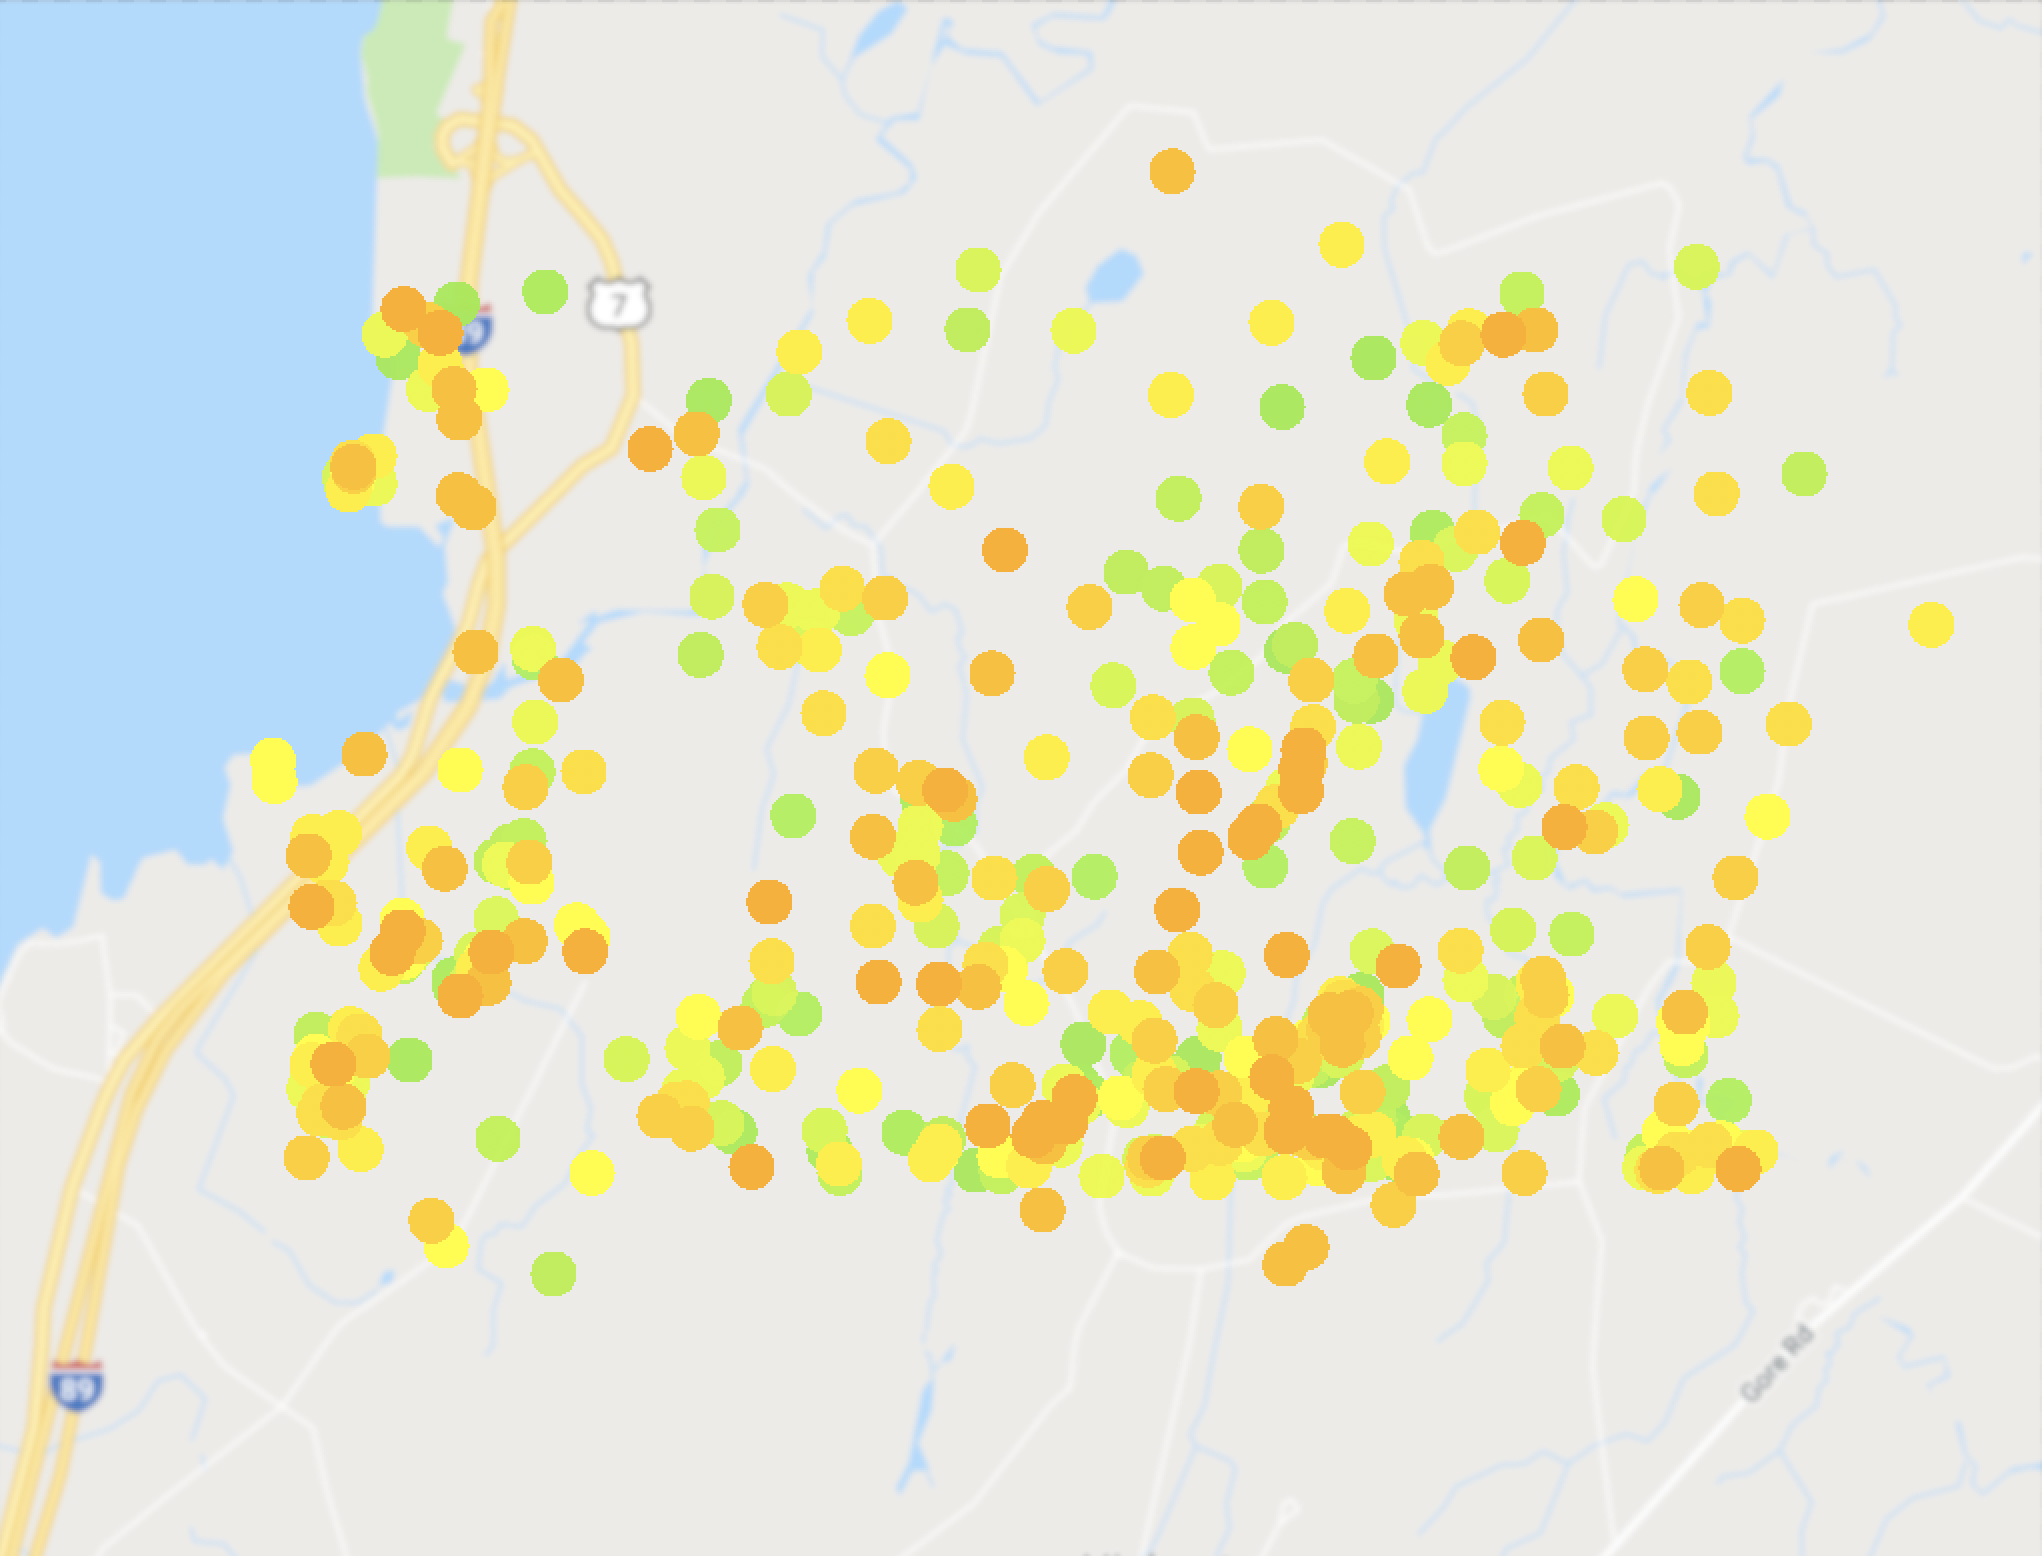
\includegraphics[width=0.45\textwidth]{figure/farm-sample-2001.png}
    \caption{A map of the study area and the locations of the agricultural
    agents within it.}
    \label{fig:app_map}
\end{figure}

\subsubsection{Agricultural Agents}

Agricultural agents model the behavior of farmers, herders, and other kinds of agricultural land managers within the study area. They make annual decisions about their farming practices, including whether they should change production in one of the four modeled agricultural industries (beef, dairy, corn, and hay) and whether they should implement an agricultural best management practice (BMP) to reduce phosphorus runoff on their land.

The state properties and variables that each agricultural agent
has are listed in Table~\ref{tab:app_farm_state}.
The initialization of these values is detailed in
Section~\ref{sec:farmer_init}.

\begin{longtable}{lll}
\caption[Table of all state properties of agricultural agents in the
farmer model]
{Table of all state properties of agricultural agents and their
associated data type for agricultural agents in this model.} \label{tab:app_farm_state} \\
\hline \hline
Name & Description & Data Type \\
\hline
\endfirsthead
\caption[]{(continued...)}\\
\hline\hline
Name & Description & Data Type \\
\hline\endhead
\hline
\endfoot
Agent ID & Unique identifier for this agent & \tt{uint} \\
Agent Status && \tt{enum\{3\}} \\
Land Parcel Data \\
\multicolumn{1}{r}{Crop Land Area $A_c$} & Land devoted to growing crops (sq km) & \tt{float} \\
\multicolumn{1}{r}{Pasture Land Area $A_p$} & Land devoted to grazing animals (sq km) & \tt{float} \\
\multicolumn{1}{r}{Total Land Area $A_{tot}$} & Total land in parcel (sq km) & \tt{float} \\
Productivity \\
\multicolumn{1}{r}{Corn $p_c$} & Corn production factor & \tt{float} \\
\multicolumn{1}{r}{Hay $p_h$} & Hay production factor & \tt{float} \\
\multicolumn{1}{r}{Beef $p_b$} & Beef production factor & \tt{float} \\
\multicolumn{1}{r}{Dairy $p_d$} & Dairy production factor & \tt{float} \\
\multicolumn{1}{r}{Phosphorous $p_{p,x}$} & Phosphorus production factor & \tt{float} \\
Cows Owned $C$ && \tt{uint} \\
Financial History \\
\multicolumn{1}{r}{Real Net} & What was net profit over last 5 years & \tt{float[5]} \\
\multicolumn{1}{r}{Expected Net} & What was expected profit for last 5 years
& \tt{float[5]} \\
Extreme Event History & Extreme event presence over past 5 years & \tt{uint[5]} \\
BMP Usage History $B$& Did farm use BMP in last 5 years & \tt{bool[5]} \\
Neighbors & References to neighboring agents & \tt{farmer*[5]} \\
Neural Networks && \\
\multicolumn{1}{r}{Actor Network $\mu$} & Network Weights & \tt{float[l][w]} \\
\multicolumn{1}{r}{Critic Network $Q$} & Network Weights & \tt{float[L][W]} \\
\multicolumn{1}{r}{Target Network $\mu'$} & Network Weights & \tt{float[l][w]} \\
\multicolumn{1}{r}{Target Network $Q'$} & Network Weights & \tt{float[L][W]} \\
Memory Bank && \tt{float[M*R]} \\
Memory Buffer && \tt{float[B*R]} \\
\end{longtable}

The components of actions that agricultural agents can take
are listed in Table~\ref{tab:app_farm_action}.

\begin{longtable}{llc}
    \caption[Table of components of actions that farmer agents can take]{Table of components of actions that farmer agents can take and their associated encoding group for $n$-hot encoding}\label{tab:app_farm_action} \\
    \hline\hline
    Group & Action & Encoding Index \\
    \hline
    \endfirsthead
    \caption[]{(continued...)}\\
    \hline\hline
    Group & Action & Encoding Index \\
    \hline
    \endhead
    \hline
    \endfoot
    \textbf{BMP Usage} & Adopt BMP & 0 \\
        & Don't Adopt BMP & 1 \\
    \textbf{Corn Production} & Increase by $[0, S^+_c)$ & 2 \\
        & Maintain & 3 \\
        & Decrease by $[0, S^-_c]$ & 4 \\
    \textbf{Hay Production} & Increase by $[0, S^+_h]$ & 5 \\
        & Maintain & 6 \\
        & Decrease by $[0, S^-_h)$ & 7 \\
    \textbf{Dairy Production} & Increase by $[0, S^+_d)$ & 8 \\
        & Maintain & 9 \\
        & Decrease by $[0, S^-_d)$ & 10 \\
    \textbf{Beef Production} & Increase by $[0, S^+_b)$ & 11 \\
        & Maintain & 12 \\
        & Decrease $[0, S^-_b)$ & 13 \\
\end{longtable}

The production factors were derived by an underlying economic model and
are calibrated from 2001--2040.
The equations used are shown for the production of corn (Eq~\ref{eq:corn}),
hay (Eq~\ref{eq:hay}),
dairy (Eq~\ref{eq:dairy}),
and beef (Eq~\ref{eq:beef}), below.

\begin{equation}
\label{eq:corn}
    P_c(t) = p_c * A_c^b * 11.433\log{t} - 86.826
\end{equation}
\begin{equation}
\label{eq:hay}
    P_h(t) = p_h * A_c^b * \SI{1e-32}{}\exp{0.0358t}
\end{equation}
\begin{equation}
\label{eq:beef}
    P_b(t) = p_b * A_p^b * \SI{2e-20}{}\exp{0.0234t}
\end{equation}
\begin{equation}
\label{eq:dairy}
    P_d(t) = p_d * A_p^b * \SI{2e-9}\exp{0.0114t}
\end{equation}

The productivity of the agent is modified by
the application of the regulatory agent's regulations $G_1$ and $G_2$
and the amount of losses due to extreme weather events (Eq~\ref{eq:stormloss})
as a function of whether the BMP was used and whether the number
of extreme events that occurred within the given year exceeds the
expected threshold~$N$.

\begin{equation}
\label{eq:stormloss}
\begin{array}{lllll}
    S(B, EE) & = & 1, & EE < N & \\
    S(B, EE) & = & 0.1, & EE \ge N, & \neg B \\
    S(B, EE) & = & (0.1 + 0.9 B_{eff}), & EE \ge N, & B \\
\end{array} 
\end{equation}

The reward function uses for training the policies of the
farmer agents (Eq~\ref{eq:farmreward})
is defined by the ratio of the squared 
realized profits of a time-step (Eq~\ref{eq:netprofit})
and the expected profits at that time-step (Eq~\ref{eq:expprofit}),
translated from the range of all possible profits $(P_{\min}, P_{\max})$
to the range $(-1, 1)$.

\begin{equation}
\label{eq:netprofit}
    P_{net}(t) = \sum_x P_x(t) G_1(P_p, B, t) S(B, EE) + G_2(P_p, B, t)
\end{equation}

\begin{equation}
\label{eq:expprofit}
    P_{exp}(t) = \sum_x P_x(t) G_1(P_p, B, t) + G_2(P_p, B, t)
\end{equation}

\begin{equation}
\label{eq:farmreward}
    R_f(t) = 
    \frac{P_{net}(t)^2}{P_{exp}(t)} 
    : \left(P_{\min}, P_{\max}\right) \rightarrow \left(-1, 1\right)
\end{equation}

\subsubsection{Regulatory Agent}

In addition to the numerous agricultural agents, the model contains 
a single regulatory agent that models 
the behavior of a municipal government or regulatory agency 
managing agricultural practices on the landscape and the local environment.
Slower acting than the agricultural agents, 
the regulator agent acts once every 5 model years, 
optionally modifying its incentive structure.

The state properties of the regulatory agent are listed in
Table~\ref{tab:app_reg_state},
and details on their initialization are included in
Section~\ref{sec:regulator_init}.

\begin{longtable}{lll}
\caption[Properties of Regulatory Agent]{Properties of Regulatory Agent}
\label{tab:app_reg_state} \\
\hline\hline
Name & Description & Data Type \\
\hline
\endfirsthead
\caption[]{(continued...)} \\
\hline\hline
Name & Description & Data Type \\
\hline
\endhead
\hline
\endfoot
Agent ID & Identifier for this agent & \tt{uint} \\
Aggregate Agent Data & & \\
\multicolumn{1}{r}{BMP Adoption} & & \tt{float[15]} \\
\multicolumn{1}{r}{Extreme Events} & & \tt{uint[15]} \\
\multicolumn{1}{r}{Financial History} & & \tt{float[15]} \\
\multicolumn{1}{r}{P Runoff History} & & \tt{float[15]} \\
\end{longtable}

The components of actions that the regulatory agent can take
are listed in Table~\ref{tab:app_reg_action}.
The phosphorus threshold adjustment action is notably implemented
differently in that it is a single value which is having the sign taken
to determine the direction of the adjustment.

\begin{longtable}{llc}
    \caption[Table of components of actions that the regulatory agent
    can take in the farm model]
    {Table of components of actions that the regulator agent can take and their associated encoding group}\label{tab:app_reg_action} \\
    \hline\hline
    Group & Action & Encoding Index \\
    \hline
    \endfirsthead
    \hline
    \endfoot
    \textbf{Tax Rate} & Increase by [0, $T^+$) & 0 \\
    & Decrease by [0, $T^-$) & 1 \\
    \textbf{BMP Subsidy} & Provide/Increase & 2 \\
    & Remove/Decrease & 3 \\
    \textbf{Phosphorous Threshold$\star$} & Scale & 4 \\
\end{longtable}

The goal of the regulator agent is to minimize the aggregate phosphorous
output and storm loss of all agricultural agents,
$R_r = \left<W_p\sum_fP_{p,f}(t), W_l\sum_fl_f\right>$,
where $W_p$ and $W_l$ are normalizing weights on the component
inverse reward signals so that they vary along ranges of similar magnitude.

\subsection{Process Overview and Scheduling}

Once every model year, starting with the first time step (t=0), 
the number of extreme weather events for the year is generated from a 
simple peaks-over-threshold weather event generator. 
The number of extreme weather events generated for the year 
impacts the agricultural agents' productivity for that year.

Agricultural agents then act every model year, 
deciding what action to take and resolving that decision on the landscape.
Every 5 model years, 
the regulator agent reads the productivity and losses from the agricultural
agents and decides how/if to alter its incentive strategy 
for adjusting agricultural agent behavior.

An overview of model execution and the looping every model
year, every 5 model years, and every training episode
is shown in Figure~\ref{fig:farm_flow}.

\begin{figure}
    \centering
    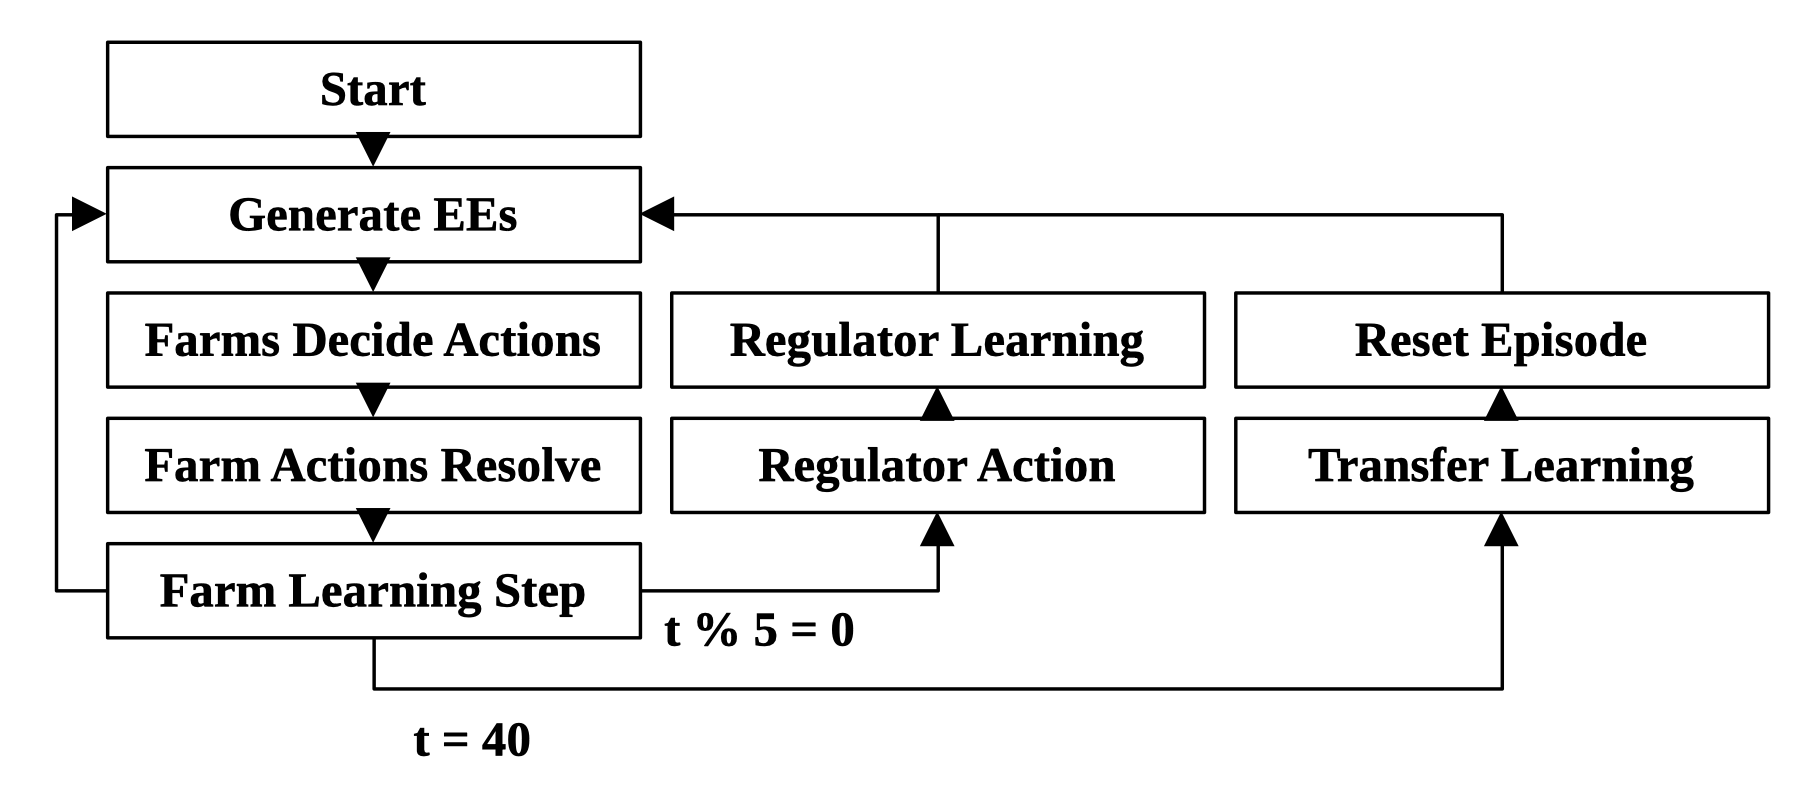
\includegraphics[width=.8\linewidth]{figure/farm-flow.png}
    \caption{A diagram of model execution throughout episodic training.
    Within each time step of the episode farmer agents make decisions
    and learn, every five time steps the regulator agent acts, and
    after 40 model years the episode ends and is reset.}
    \label{fig:farm_flow}
\end{figure}

\section{Design Concepts}

\subsection{Basic Principles}
This model is an agent-based model where the agents exist on a shared grid
representative of the chosen study area. 
Each agent has control over a portion of this grid as defined by 
parcel boundaries and can make decisions that can alter the
productivity and land-use practices of the land they manage. 
Agents take actions independently, 
and their effect on the grid is synchronized at the end of every time step.

Agents create their decision-making policies 
using deep reinforcement learning, 
where environmental feedback and internal reward valuation 
drive the way their internal neural networks learn. 
Additionally, as they act, state-transitions are stored as memories 
within the agents, 
which are used to determine an agent's learning speed 
and verify that learning progresses in the right direction.

\subsection{Emergence}

There are a few areas of the model where interesting behavioral patterns are more likely to emerge and be observed. The most visible way is how the agricultural agents adopt/reject best management practices on their land. Their choices are also directly observed and recorded, which allows for the observation of behavioral trends over time and how those trends correlate to factors like the number of extreme weather events that occur per model year.

\subsection{Adaptation}

Agents have a few different adaptive traits,
viz. the neural networks used to drive agent decision-making.
The networks take in components of the agents' current state 
and use them to select an action to take, 
over time encoding the agents' decision-policies 
and their reward valuation into the networks.

Additionally, 
the agricultural agents have several features related 
to agricultural production and BMP usage, 
which factor into their decision-making and can be adjusted over time.

\subsection{Objectives}
The two agent types have distinct, 
somewhat adversarial objectives with regard to adapting their 
decision-making.
Both agent types are working towards optimizing their reward functions
and associated valuation accuracy.

The goal of the agricultural agents is to maximize their yearly profits.
The goal of the regulatory agent is to minimize the aggregate storm loss
accrued by the farmer agents and their aggregate phosphorous output.

\subsection{Learning}

All human agents in the model learn and develop their decision-making 
policies using deep reinforcement machine learning,
specifically an adapted version of DDQN. 
As the agents take actions in various states and transition between them,
these state transitions are stored in the agents' memory.
After resolving an action,
the most recent state transition is compared against state transitions 
in agent memory to determine the direction 
and rate of learning within the problem space. 
The gradient generated from this calculation is then used 
to adjust the agents' neural networks' weights and 
steer their decision-policy towards selecting actions 
that will create state transitions most in line with their objectives.

\subsection{Prediction}

Because of how the internal neural networks work, the prediction of future state-transitions is an implicitly defined process. As each agent makes decisions and experiences state transitions, it updates a valuation network that estimates the value of taking actions from states. This estimated valuation is compared against the actual reward received from taking that action, which is used to update the decision-making network. Because the actual value of taking an action will not be known until the action resolves on the landscape, the prediction is somewhat retroactively validated and used to drive network learning, as opposed to being used to explicitly and actively look forward while decision-making.

\subsection{Sensing}
\label{sec:farm_sensing}

Agricultural agents are capable of detecting some historical information about storm productivity losses and BMP usage from the five nearest neighboring agents. They also experience extreme weather events as they occur during model years, affecting their yearly productivity.
The regulator agent can read information about the state of the agricultural agents as a collective group and can communicate a uniform regulatory policy to the agricultural agents.
These data fields are listed in Table~\ref{tab:app_farm_sensing}.

\begin{longtable}{lllll}
\caption[Table listing information shared between agents in the farm model]{A listing of information shared between agents in this model and its directionality}\label{tab:app_farm_sensing} \\
\hline\hline
Value & From & To & Type \\
\hline
\endhead
\hline\endfoot
BMP Usage (5-year) & Farmers & 5-nearest Neighbors & \tt{bool[5]} \\
Net Profits/Losses (5-year) & Farmers & 5-nearest Neighbors & \tt{float[5]} \\
BMP Usage & Farmers & Regulator & \tt{bool} \\
Net Profits/Losses & Farmers & Regulator & \tt{float} \\
P Output & Farmers & Regulator & \tt{float} \\
Losses (1-year) & 
\end{longtable}

\subsection{Interaction}

Agents in this model neither communicate nor interact with one another
directly;
they do however passively share information as outlined 
in Section~\ref{sec:farm_sensing}.
Additionally, the regulator agent has the ability to change the
reward/incentive structure for the agriculture agents when it acts on
5-year intervals.

\subsection{Stochasticity}

Randomness is used in multiple components of the model. During agent initialization, triangle distributions generate the starting productivity for the agricultural agents, and He network initialization is used to set the initial neural network weights, which are detailed in Section~\ref{sec:farmer_init}.

During training runs of the model, memories are selected as a basis buffer for learning using a uniform distribution. Additionally, in runs with nonzero forgetfulness factors, a degree of uniform stochasticity is added to the accuracy of memory recall proportional to the factor.

\subsection{Collectives}

Agricultural agents share some historical information with their
5-nearest neighbors,
as outlined in Section~\ref{sec:farm_sensing},
but generally aren't collected in any higher ordered structuring
outside of network analysis.

\subsection{Observation}

Several components of the model are tracked during runs and compiled
as observational data.
Agent decisions, farmer budgets, and overall network training/performance
are recorded throughout model runs.

\section{Details}

\subsection{Initialization}

Several of the parameters are initialized according 
to triangular distributions, seen below.
Neural networks had weights initialized according to the He~initialization
algorithm.~\cite{he2004initialization}.

\newcommand{\Tri}[0]{\text{Tri}}

\begin{equation}
\label{eq:tri}
    \Tri_1\left(a, b, c\right)
    = \left\{
    \begin{array}{ll}
    a + \sqrt{U (b - a) (c - a)} & \text{for } 0 < U < F(c) \\
    b - \sqrt{(1 - U) (b - a) (b - c)} & \text{for } F(c) \le U < 1 \\
    \end{array}
    \right.
\end{equation}
\begin{equation}
    \Tri_2\left(a, b\right) = 
    \Tri_1\left(a, b, \frac{a}{b}\right)
\end{equation}
\begin{equation}
    \Tri_3\left(\mu, \delta\right) = 
    \Tri_1\left(\mu-\delta, \mu+\delta, \mu\right)
\end{equation}

\subsubsection{Farmer Agents}
\label{sec:farmer_init}
Many of the initial values used by the agricultural agents are initialized
from the input data.
The variables which are set during initialization are listed in
Table~\ref{tab:farmer_init}.
Many of these values are selected from a triangular distribution
which was parameterized according to the calibration of the
underlying economic model.

\begin{longtable}{lcll}
    \caption[Table listing initialization of parameters of
    the agricultural agents in the farm model]
    {Initialization of Farm Agents}
    \label{tab:farmer_init}
    \\
    \hline\hline
    Value & & Initialization & Type \\
    \hline
    \endfirsthead
    \caption[]{(continued ...)}\\ \hline\hline
    Value & & Initialization & Type\\ \hline
    \endhead
    \hline
    \endfoot
    Agent ID & $f$ & Assigned sequentially from 0 & \tt{uint} \\
    Parcel Data & $A_x$ & 
    Read from input file & \tt{float} \\
    Corn Production (USD) & $p_c$ 
        & $\Tri_2(3.362551, 4259232)$ & \tt{float} \\
    Corn Production (P) & $p_{p,c}$ 
        & $\Tri_2(\SI{2.02e-4}{}, \SI{6.17e-4}{})$ & \tt{float} \\
    Hay Production (USD) & $p_h$ 
        & $\Tri_2(0.358672, 0.470757)$ & \tt{float} \\
    Hay Production (P) & $p_{p,h}$
        & $\Tri_2(\SI{3.37e-5}{}, \SI{1.12e-4}{})$ & \tt{float} \\
    Beef Production (USD) & $p_b$ & $\Tri_2(900.0, 1200.0)$ & \tt{float} \\
    Dairy Production (USD) & $p_d$ & $\Tri_2(210.0, 250.0)$ & \tt{float} \\
    Cow Production (P) & $p_{p,[bd]}$ 
        & $\Tri_2(\SI{3.366e-4}{}\SI{7.853e-4}{})$ & \tt{float} \\
    Cows Owned & $C$ & $\Tri_2(3600, 7800)$ & \tt{uint} \\
    Actor-Network Weights & $\Theta_\mu$ & He() & \tt{float[][]} \\
    Critic-Network Weights & $\Theta_Q$ & He() & \tt{float[][]} \\
    Target-Actor Weights & $\Theta_{\mu'}$ 
        & Copied from $\Theta_\mu$ & \tt{float[][]} \\
    Target-Critic Weights & $\Theta_{Q'}$ 
        & Copied from $\Theta_Q$ & \tt{float[][]} \\
\end{longtable}

\subsubsection{Regulatory Agent}
\label{sec:regulator_init}

The regulatory agent is more reactive than proactive,
so most of its internal parameters cannot be set until after
the agricultural agents have began to act;
however, the parameters that are generated during initialization are
listed in Table~\ref{tab:regulator_init}.

\begin{longtable}{lcll}
    \caption[Table listing initialization of parameters of
    the regulatory agent in the farm model]
    {Initialization of Regulatory Agent}
    \label{tab:regulator_init}
    \\
    \hline\hline
    Value & & Initialization & Type \\
    \hline
    \endfirsthead
    \caption[]{(continued ...)}\\ \hline\hline
    Value & & Initialization & Type\\ \hline
    \endhead
    \hline
    \endfoot
    Agent ID & $r$ & Only 1, so set to 0 & \tt{uint} \\
    Actor-Network Weights & $\Theta_\mu$ & He() & \tt{float[][]} \\
    Critic-Network Weights & $\Theta_Q$ & He() & \tt{float[][]} \\
    Target-Actor Weights & $\Theta_{\mu'}$ 
        & Copied from $\Theta_\mu$ & \tt{float[][]} \\
    Target-Critic Weights & $\Theta_{Q'}$ 
        & Copied from $\Theta_Q$ & \tt{float[][]} \\
\end{longtable}
